\chapter{Eksploracja danych}
\label{sec:eksploracja}

W niniejszym rozdziale przedstawiono proces przygotowania omówionego zestawu danych. Proces eksploracji danych obejmuje obsługę braków wartości, dostosowanie rozdzielczości zmiennych, analizę korelacji, podział danych na okresy o różnej zmienności, podział na zbiory treningowy i testowy oraz preprocessing danych przed modelowaniem.

\section{Wstępna obróbka danych}
\subsubsection{Obsługa braków wartości}
Pierwszym etapem eksploracji danych jest analiza i obróbka brakujących wartości w zbiorze danych, co stanowi kluczowy krok w zapewnieniu jego jakości dla dalszej analizy. Brakujące wartości (NaN) w zmiennych objaśniających mogą wynikać z braku pomiarów w określonych godzinach, błędów w procesie gromadzenia danych lub ich celowego pominięcia. Początkowa ocena wykazała obecność 830 brakujących wartości oraz 120 zduplikowanych w zbiorze danych, który docelowo powinien obejmować 70128 rekordów godzinowych. Łączna liczba zduplikowanych i brakujących rekordów (950) stanowiła 1.35\% w stosunku do oczekiwanej liczby rekordów.

Brakujące wartości rzadko stanowiły okres dłuższy, niż dwie godziny. Z tego powodu, w procesie obróbki zastosowano interpolację liniową do wypełnienia brakujących wartości, zapewniając ciągłość danych w ujęciu godzinowym. 120 zduplikowanych timestampów, z których usunięto drugie wystąpienie każdej pary, co pozwoliło na uzyskanie unikalnego zbioru 70128 rekordów. Takie podejście zminimalizowało utratę informacji i zapewniło spójność danych, umożliwiając ich dalsze wykorzystanie w modelowaniu.

\subsubsection{Obsługa różnic w rozdzielczości danych}
Dane użyte w pracy charakteryzowały się różną rozdzielczością czasową. PSE udostępnia dane dotyczące sieci energii elektrycznej, w tym handlu w rozdzielczości godzinowej. Zmienne pogodowe również mają rozdzielczość dzienną. Natomiast zmienne makroekonomiczne, takie jak ceny paliw, są dostępne w częstotliwości dniowej lub tygodniowej.

Aby ujednolicić rozdzielczość do poziomu godzinowego, zastosowano dwie techniki. W przypadku zmiennych o rozdzielczości dziennej, takich jak ceny gazu ziemnego, założono, że wartości w ciągu doby nie ulegają zmianie. Wartości dzienne przypisano więc każdej godzinie danego dnia, co pozwoliło na zachowanie prostoty przy jednoczesnym dostosowaniu danych do godzinowej rozdzielczości ceny energii. 

Dla zmiennych o rzadszej rozdzielczości, na przykład dla ceny węgla (miesięczna) oraz emisji CO2 (tygodniowa), przeprowadzono uzupełnianie danych metodą interpolacji liniowej między sąsiednimi wartościami. Poniższy przykład dla rozdzielczości tygodniowej.
\[
\text{cena w dniu } d = \text{cena w tygodniu } t + \left( \frac{\text{cena w tygodniu } t+1 - \text{cena w tygodniu } t}{6} \right) \times d
\]
, gdzie \( \quad d \in [t, t+1] \) \newline
Następnie, podobnie jak w przypadku danych dziennych, wartości te przypisano każdej godzinie w danej dobie. Podejście to umożliwiło ujednolicenie wszystkich zmiennych do godzinowej rozdzielczości danych docelowych.

\section{Analiza korelacji}

Aby zbadać zależności między zmiennymi objaśniającymi a zmienną docelową, przeprowadzono analizę korelacji, wykorzystując dwa współczynniki: Pearsona i Spearmana. Wybór odpowiedniego współczynnika dla każdej zmiennej oparto na charakterze jej relacji z \texttt{fixing\_i\_price}, co pozwoliło na bardziej precyzyjne oszacowanie siły i rodzaju zależności.

Współczynnik korelacji Pearsona (\( r \)) mierzy liniową zależność między dwiema zmiennymi. Jest on zdefiniowany wzorem:
\[
r = \frac{\sum_{i=1}^{n} (x_i - \bar{x})(y_i - \bar{y})}{\sqrt{\sum_{i=1}^{n} (x_i - \bar{x})^2} \sqrt{\sum_{i=1}^{n} (y_i - \bar{y})^2}},
\]
gdzie \( x_i \) i \( y_i \) to wartości zmiennych i danej zmiennej objaśniającej), \( \bar{x} \) i \( \bar{y} \) to ich średnie, a \( n \) to liczba obserwacji. Współczynnik Pearsona przyjmuje wartości w przedziale \([-1, 1]\), gdzie \( r = 1 \) oznacza doskonałą dodatnią zależność liniową, \( r = -1 \) doskonałą ujemną zależność liniową, a \( r = 0 \) brak liniowej zależności.

Pearson jest odpowiedni dla zmiennych, których relacja jest liniowa. Na przykład wzrost zapotrzebowania zwykle większa ceny energii liniowo.

Współczynnik korelacji Spearmana (\( \rho \)) mierzy monotoniczną zależność między zmiennymi, co czyni go bardziej odpowiednim dla relacji nieliniowych. Spearman opiera się na rangach wartości zmiennych, a jego wzór to:

\[
\rho = 1 - \frac{6 \sum_{i=1}^{n} d_i^2}{n(n^2 - 1)},
\]

gdzie \( d_i \) to różnica między rangami wartości \( x_i \) i \( y_i \). Współczynnik Spearmana również przyjmuje wartości w przedziale \([-1, 1]\), ale nie zakłada liniowości relacji - wystarczy, że wzrost jednej zmiennej odpowiada wzrostowi (lub spadkowi) drugiej w sposób monotoniczny.

Spearman jest szczególnie użyteczny dla zmiennych o nieliniowej relacji z \texttt{fixing\_i\_price}. Na przykład wzrost cen gazu w 2022 roku prowadził do nieproporcjonalnego wzrostu cen energii, co lepiej oddaje Spearman niż Pearson.

W celu wyboru odpowiedniego współczynnika korelacji obliczono zarówno korelację Pearsona, jak i Spearmana dla wszystkich zmiennych objaśniających względem \texttt{fixing\_i\_price}. Następnie obliczono bezwzględną różnicę między tymi współczynnikami (\(| \rho - r |\)). Zmienne, dla których różnica była większa niż 0,1, uznano za posiadające nieliniową relację z \texttt{fixing\_i\_price}, stosując dla nich korelację Spearmana. W pozostałych przypadkach wybrano korelację Pearsona, zakładając liniową zależność. 

Analiza wykazała, że zmienne takie jak \texttt{co2\_price} (różnica 0,114), \texttt{coal\_pscmi1\_pln\_per\_gj} (0,161), \texttt{pln\_usd} (0,112), \texttt{solar} (0,172), \texttt{gas} (0,153), \texttt{biomass} (0,174), \texttt{coal-derived} (0,142) oraz zmienne związane z promieniowaniem słonecznym (różnice 0,106-0,115) mają nieliniową relację z \texttt{fixing\_i\_price}. Nieliniowość wynika z charakteru tych zmiennych - na przykład wysoka produkcja energii z fotowoltaiki w miesiącach letnich obniża ceny energii w sposób nieproporcjonalny, co prowadzi do bardzo niskich, a czasem ujemnych cen. Podobnie gwałtowny wzrost cen CO2 w okresie niespokojnym (2020-2023) zwiększał koszty produkcji energii w elektrowniach węglowych, ale efekt ten był wzmacniany przez inne czynniki, takie jak spekulacje rynkowe.

W wyniku tego powstał następujący wykres korelacji poniżej

\begin{figure}[H]
    \centering
    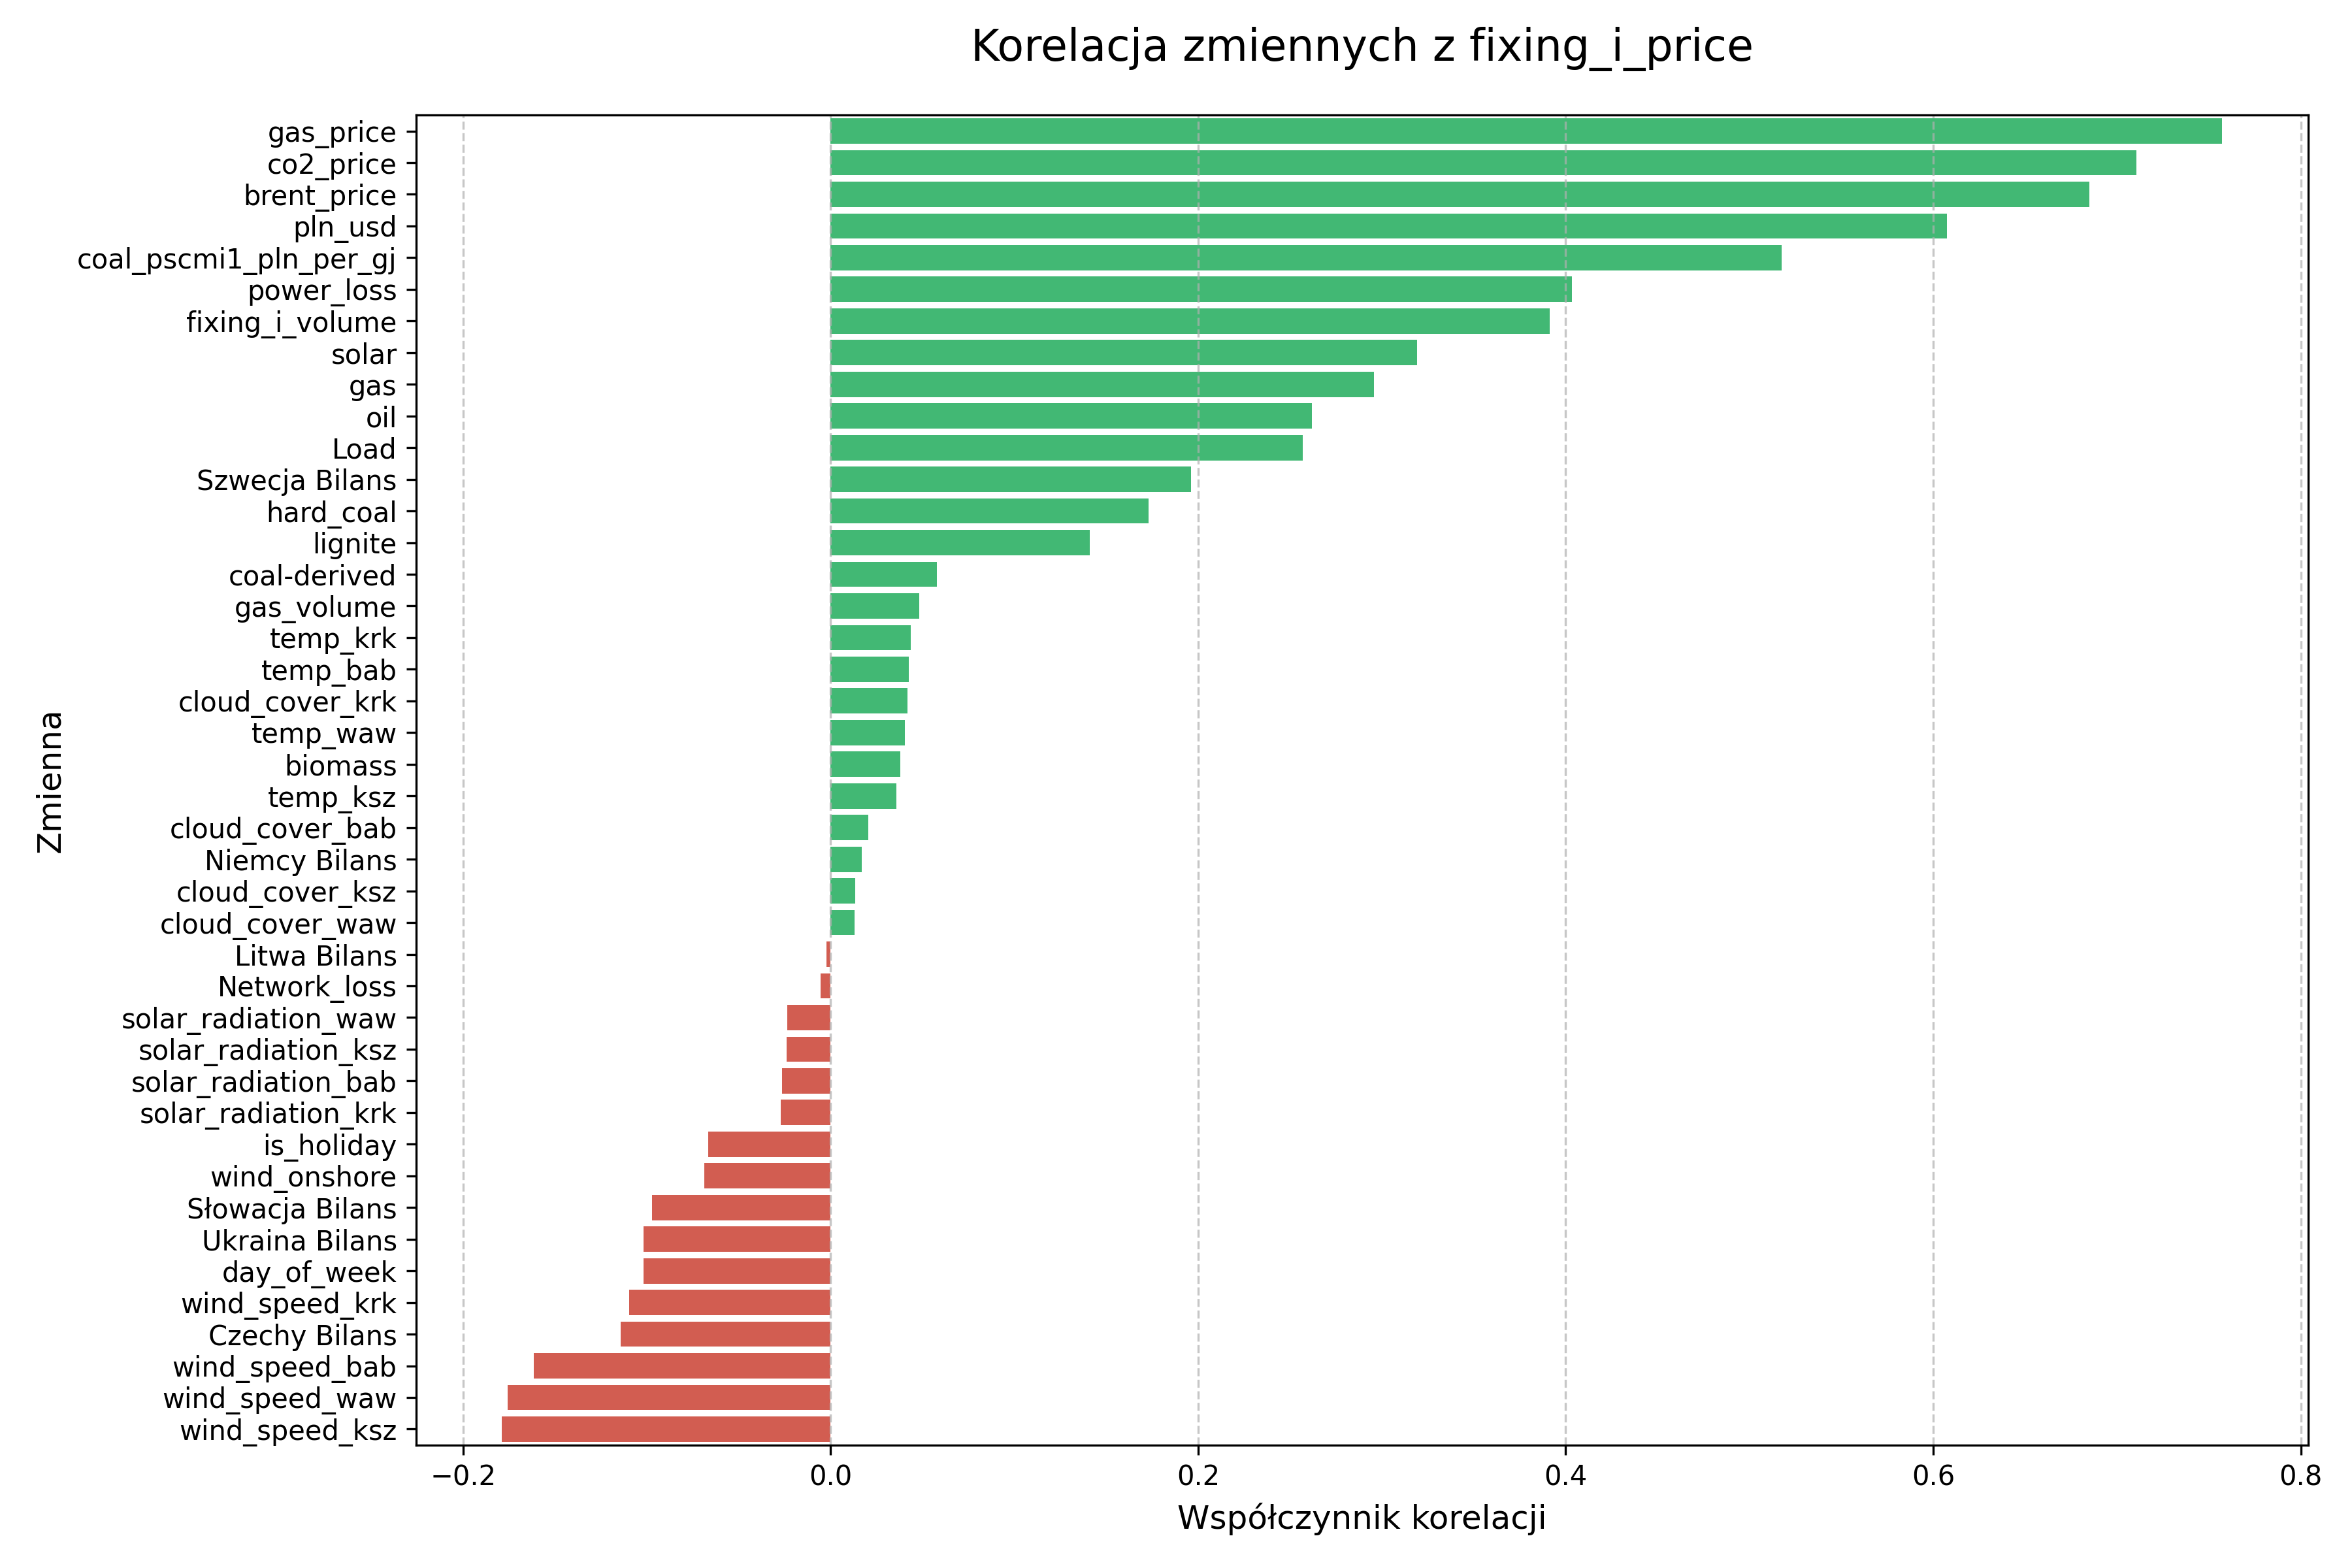
\includegraphics[width=0.9\textwidth]{../plots/correlation_with_fixing_i_price.png}
    \caption{Wykres korelacji zmiennych objaśniających względem zmiennej docelowej \texttt{fixing\_i\_price}. Opracowanie własne.}
    \label{fig:correlation_plot}
\end{figure}

Największą korelację ze zmienną objaśnianą mają zmienne reprezentujące ceny, takie jak ceny na RB, ceny na rynkach sąsiednich, ceny opóźnione oraz średnie kroczące. Kolejnymi zmiennymi wykazującymi silną korelację są ceny na surowce, kurs polskiego złotego oraz zapotrzebowanie i wolumen. Sprzeczna z logiką może być pozytywna korelacja ceny z zmienną \texttt{solar}, która wskazuje na produkcję energii z paneli fotowoltaicznych. Wynika to prawdopodobnie z faktu, w momentach, gdy świeci słońce i produkcja energii z OZE jest wysoka, zapotrzebowanie również jest zwiększone i to powoduje wzrost cen. Z kolei wartości reprezentujące parametry pogodowe nie wykazują istotnej korelacji. 

Produkcja energii z odnawialnych źródeł i gazu również odgrywa rolę. Zmienna \texttt{solar} (Spearman: 0,490) wskazuje, że wysoka produkcja energii z fotowoltaiki obniża ceny energii, szczególnie w miesiącach letnich, gdzie nadpodaż energii z OZE może prowadzić do bardzo niskich cen. \texttt{gas} (Spearman: 0,449) pokazuje, że produkcja energii z gazu ma nieliniowy wpływ, zależny od cen gazu i dostępności innych źródeł energii. Ponadto zmienne takie jak \texttt{fixing\_i\_volume} (Spearman: 0,442), \texttt{power\_loss} (Spearman: 0,441), \texttt{oil} (Spearman: 0,349) oraz \texttt{Load} (Pearson: 0,256) mają umiarkowany wpływ, odzwierciedlając znaczenie wolumenu obrotu, strat w sieci, produkcji z oleju oraz zapotrzebowania na energię.

\subsubsection{Zbiór danych skrócony}
\label{sec:shortened_dataset}
Na podstawie analizy korelacji stworzony został skrócony zbiór danych, który z pierwotnych 54 regresorów zostawia najbardziej istotne. Tymi zmiennymi zostały wszystkie przekraczające próg istotności na poziomie \texttt{0.2}, zmienne sezonowe określające dzień tygodnia, miesiąc, godzinę oraz święta, średnia arytmetyczna ze zmiennych objaśniających prędkość wiatru w Polsce, gdyż wykazują one najmocniejszą odwrotną korelację oraz zmienna objaśniająca generację OZE w procentach, ponieważ jest to ważna zmienna z punktu widzenia literatury. W wyniku tego powstał zbiór danych z 33 zmiennymi objaśniającymi. Taki zbiór danych został określony jako \texttt{zbiór danych skrócony} i będzie użyty w dalszej części pracy do analizy w celu sprawdzenia istotności zbioru danych o największej ilości parametrów. Poniżej przedstawiono mapę cieplną dla zmiennych objaśniających w zbiorze danych skróconym bez uwzględnienia zmiennych opóźnionych i średnich. 

\begin{figure}[H]
    \centering
    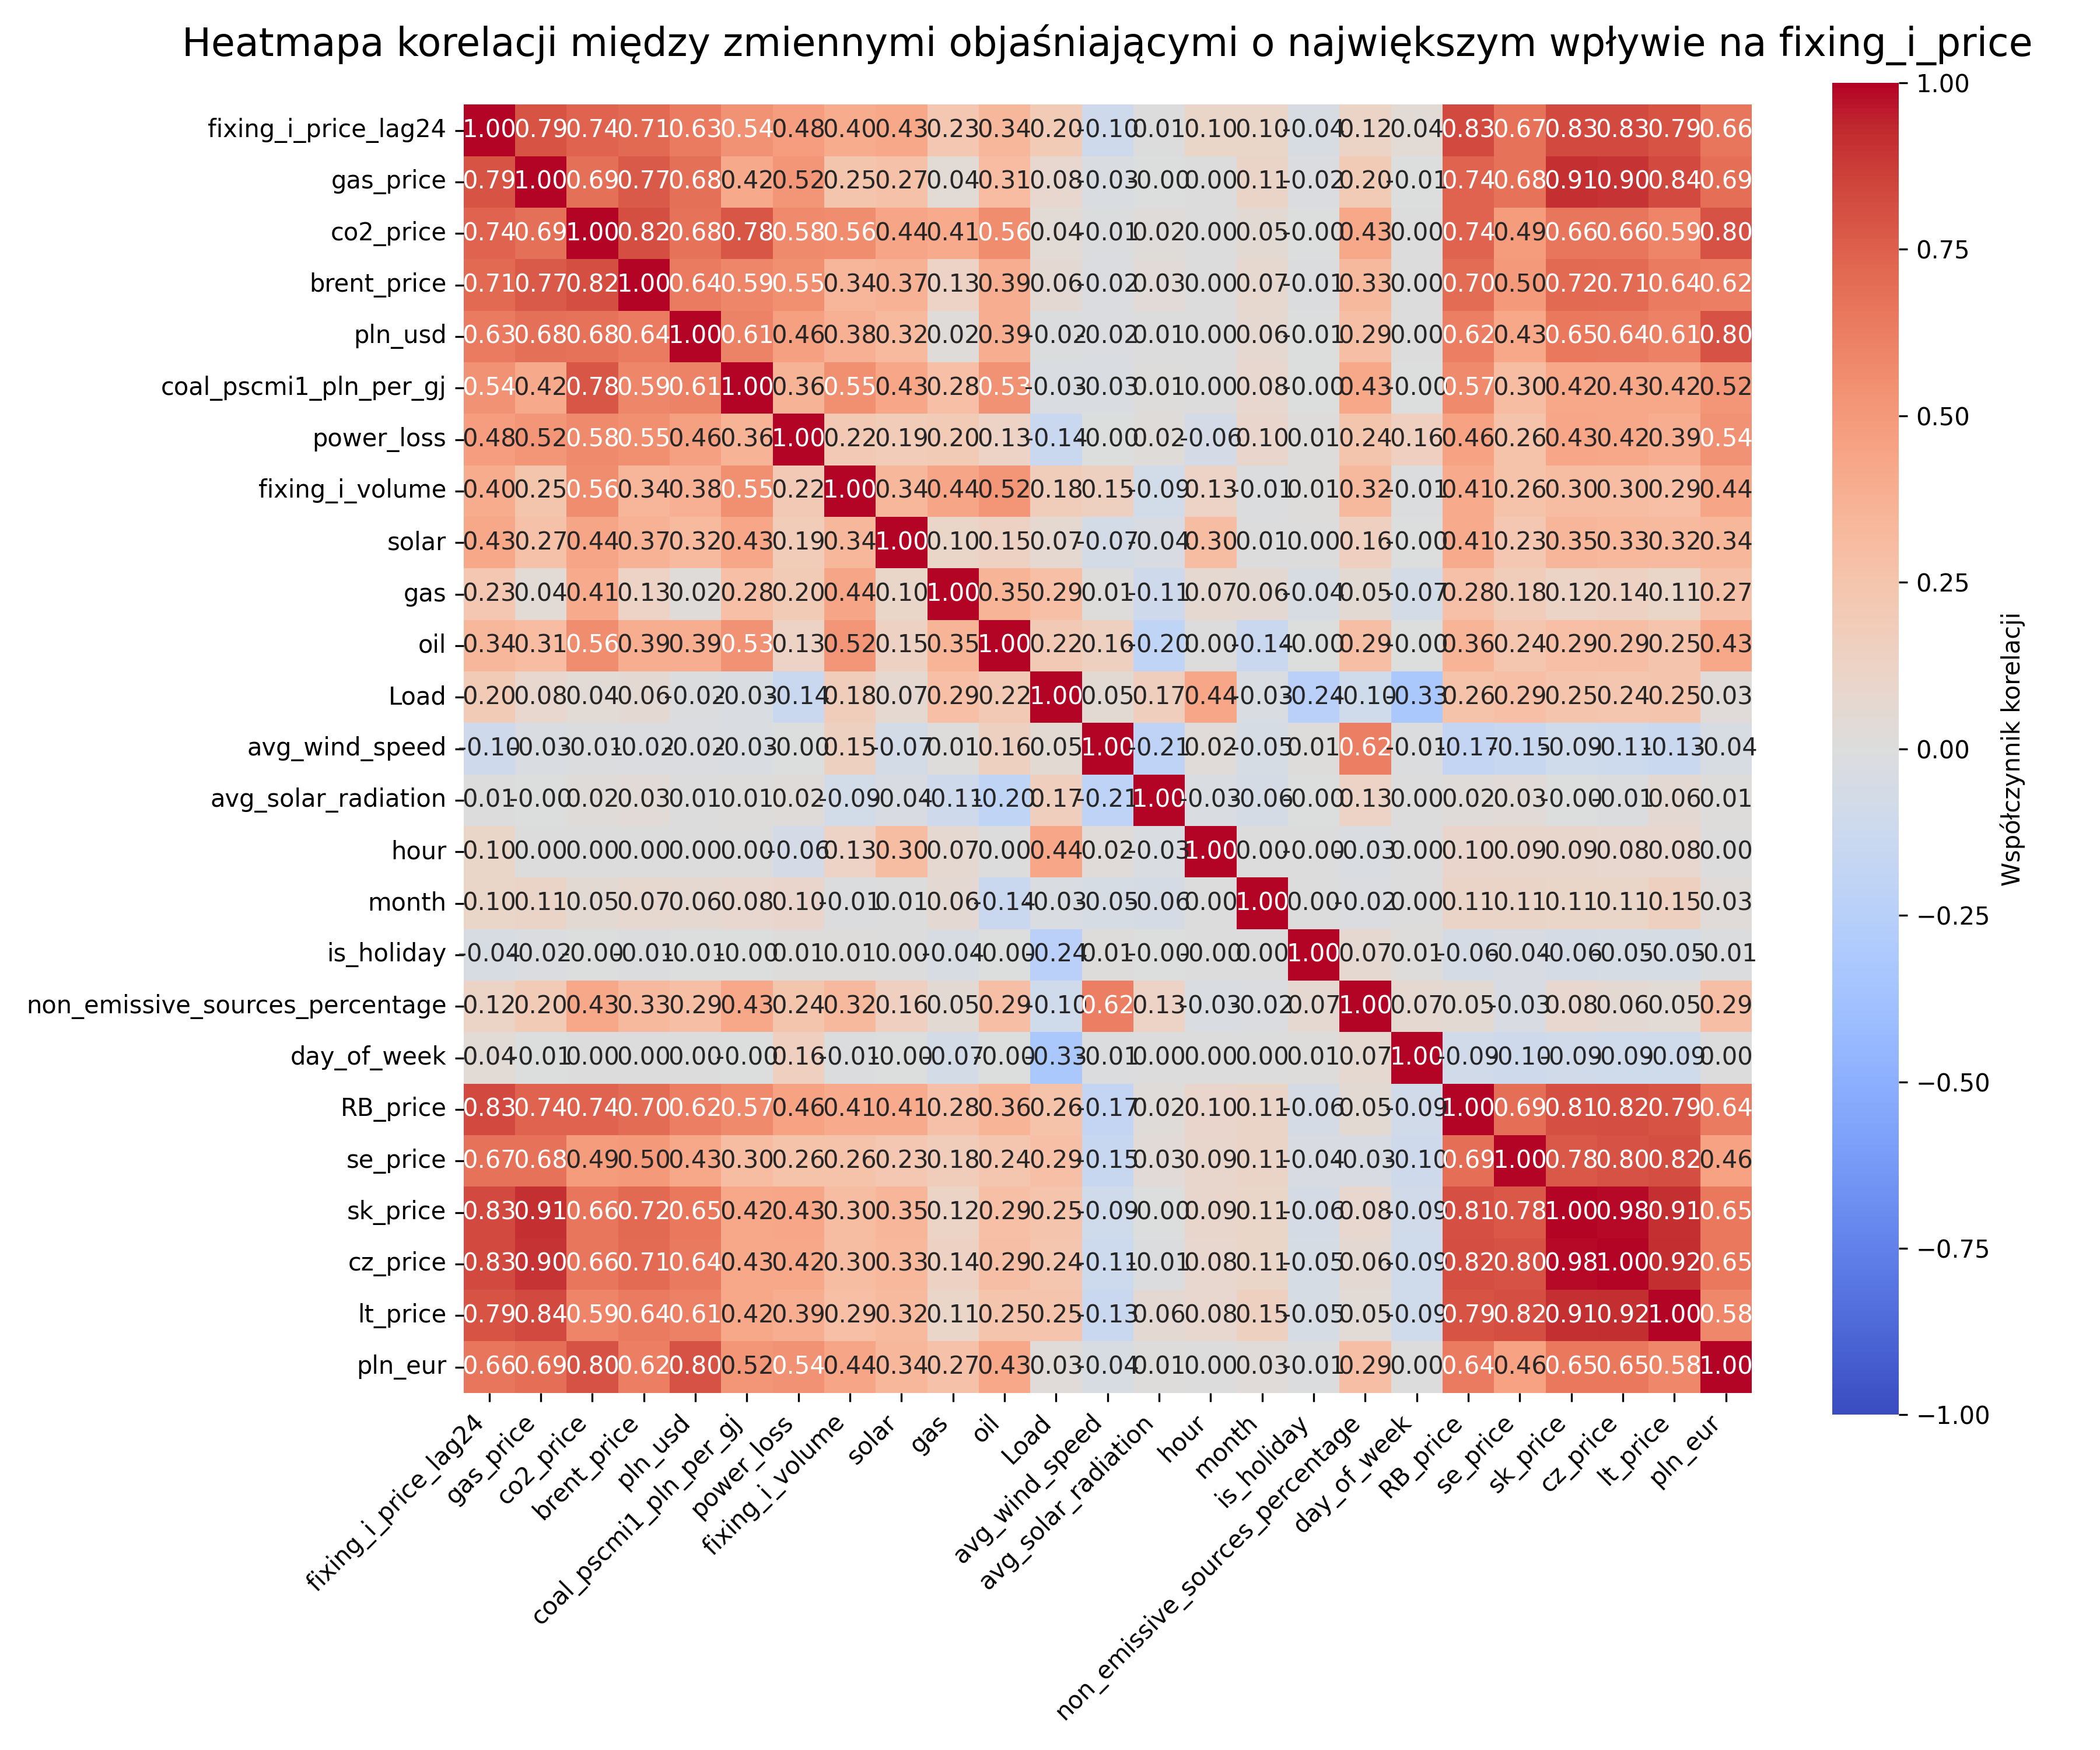
\includegraphics[width=0.9\textwidth]{../plots/heatmap_short_db_features.png}
    \caption{Mapa cieplna korelacji zmiennych objaśniających w skróconym zbiorze danych. Opracowanie własne.}
    \label{fig:heatmap_shortened_dataset}
\end{figure}

Z powyższej mapy cieplnej wynika, że zmienne o największej korelacji z ceną energii w dużym stopniu są również skorelowane pomiędzy sobą. 

\section{Podział danych}

\subsubsection{Podział na okresy spokojny i niespokojny}

Dane zostały podzielone na dwa okresy w celu uwzględnienia różnych warunków rynkowych i ich wpływu na ceny energii. Okres spokojny (2016-2019) charakteryzuje się stabilnymi cenami energii, wynikającymi z braku znaczących szoków podażowych, łatwiej przewidywalnych cen paliw oraz łagodnego wzrostu cen CO2 w ramach polityki klimatycznej UE. W tym okresie nie występowały większe kryzysy geopolityczne ani pandemie, co pozwoliło na utrzymanie cen w stosunkowo wąskim zakresie.

Okres niespokojny (2020-2023) został zdominowany przez szereg wydarzeń, które drastycznie wpłynęły na rynek energii. Pandemia COVID-19 w latach 2020-2021 początkowo obniżyła zapotrzebowanie na energię, ale ożywienie gospodarcze w 2021 roku spowodowało gwałtowny wzrost cen. Kryzys energetyczny w latach 2021-2022, związany z ograniczoną podażą gazu, rekordowymi cenami CO2 oraz wysokimi cenami węgla, doprowadził do ekstremalnych skoków cen energii. Wybuch wojny na Ukrainie w 2022 roku dodatkowo zaostrzył sytuację, powodując przerwanie dostaw gazu z Rosji, sankcje i spekulacje rynkowe, co przełożyło się na rekordowe ceny energii. W tym okresie pojawiły się również ujemne ceny, wynikające z nadpodaży energii z OZE i ograniczonej elastyczności systemu elektroenergetycznego.

Statystyki opisowe dla obu okresów przedstawiono w tabeli~\ref{tab:periods_stats_comparison}. Okres spokojny charakteryzuje się niższą średnią ceną, mniejszą zmiennością i dużo mniejszym odchyleniem standardowym, co odzwierciedla stosunkowo stabilne warunki rynkowe. W okresie niespokojnym średnia cena wzrosła, a współczynnik zmienności i odchylenie znacząco rosną. W latach 2020-2023 pojawiły się również ujemne ceny oraz rekordowe maksima. Podział na te dwa okresy i poddanie ich osobnej analizie pozwoli lepiej ocenić skuteczność wybranych cech i modeli w różnych warunkach rynkowych.

\begin{table}[h]
    \centering
    \caption{Porównanie statystyk opisowych cen energii w okresach spokojnym (2016-2019) i niespokojnym (2020-2023).}
    \label{tab:periods_stats_comparison}
    \begin{tabular}{|l|c|c|}
        \hline
        \textbf{Miara} & \textbf{Okres spokojny} & \textbf{Okres niespokojny} \\
        \hline
        Średnia (PLN/MWh) & 193,51 & 478,06 \\
        \hline
        Mediana (PLN/MWh) & 182,00 & 412,00 \\
        \hline
        Odchylenie standardowe (PLN/MWh) & 70,67 & 321,39 \\
        \hline
        Współczynnik zmienności (\%) & 36,52 & 67,23 \\
        \hline
        Kwartyl Q1 (25\%) (PLN/MWh) & 143,66 & 246,41 \\
        \hline
        Kwartyl Q3 (75\%) (PLN/MWh) & 229,35 & 609,00 \\
        \hline
        Minimum (PLN/MWh) & 31,00 & -50,00 \\
        \hline
        Maksimum (PLN/MWh) & 1199,53 & 3812,45 \\
        \hline
        Procent dni z ceną powyżej 500 PLN/MWh (\%) & 0,41 & 36,94 \\
        \hline
    \end{tabular}
\end{table}

\subsubsection{Podział danych na zbiory treningowe i testowe}

Dane zostały podzielone na zbiory treningowe i testowe w obrębie każdego z dwóch okresów, aby uwzględnić strukturę szeregów czasowych. Podział został przeprowadzony sekwencyjnie w proporcji 75/25, co zapewnia dużą ilość danych do treningu (3 lata) oraz odpowiednią ilość danych do testowania (1 rok). W przypadku takiego podziału w zbiorach testowych można przetestować wszystkie okresy sezonowe.

\begin{figure}[h]
    \centering
    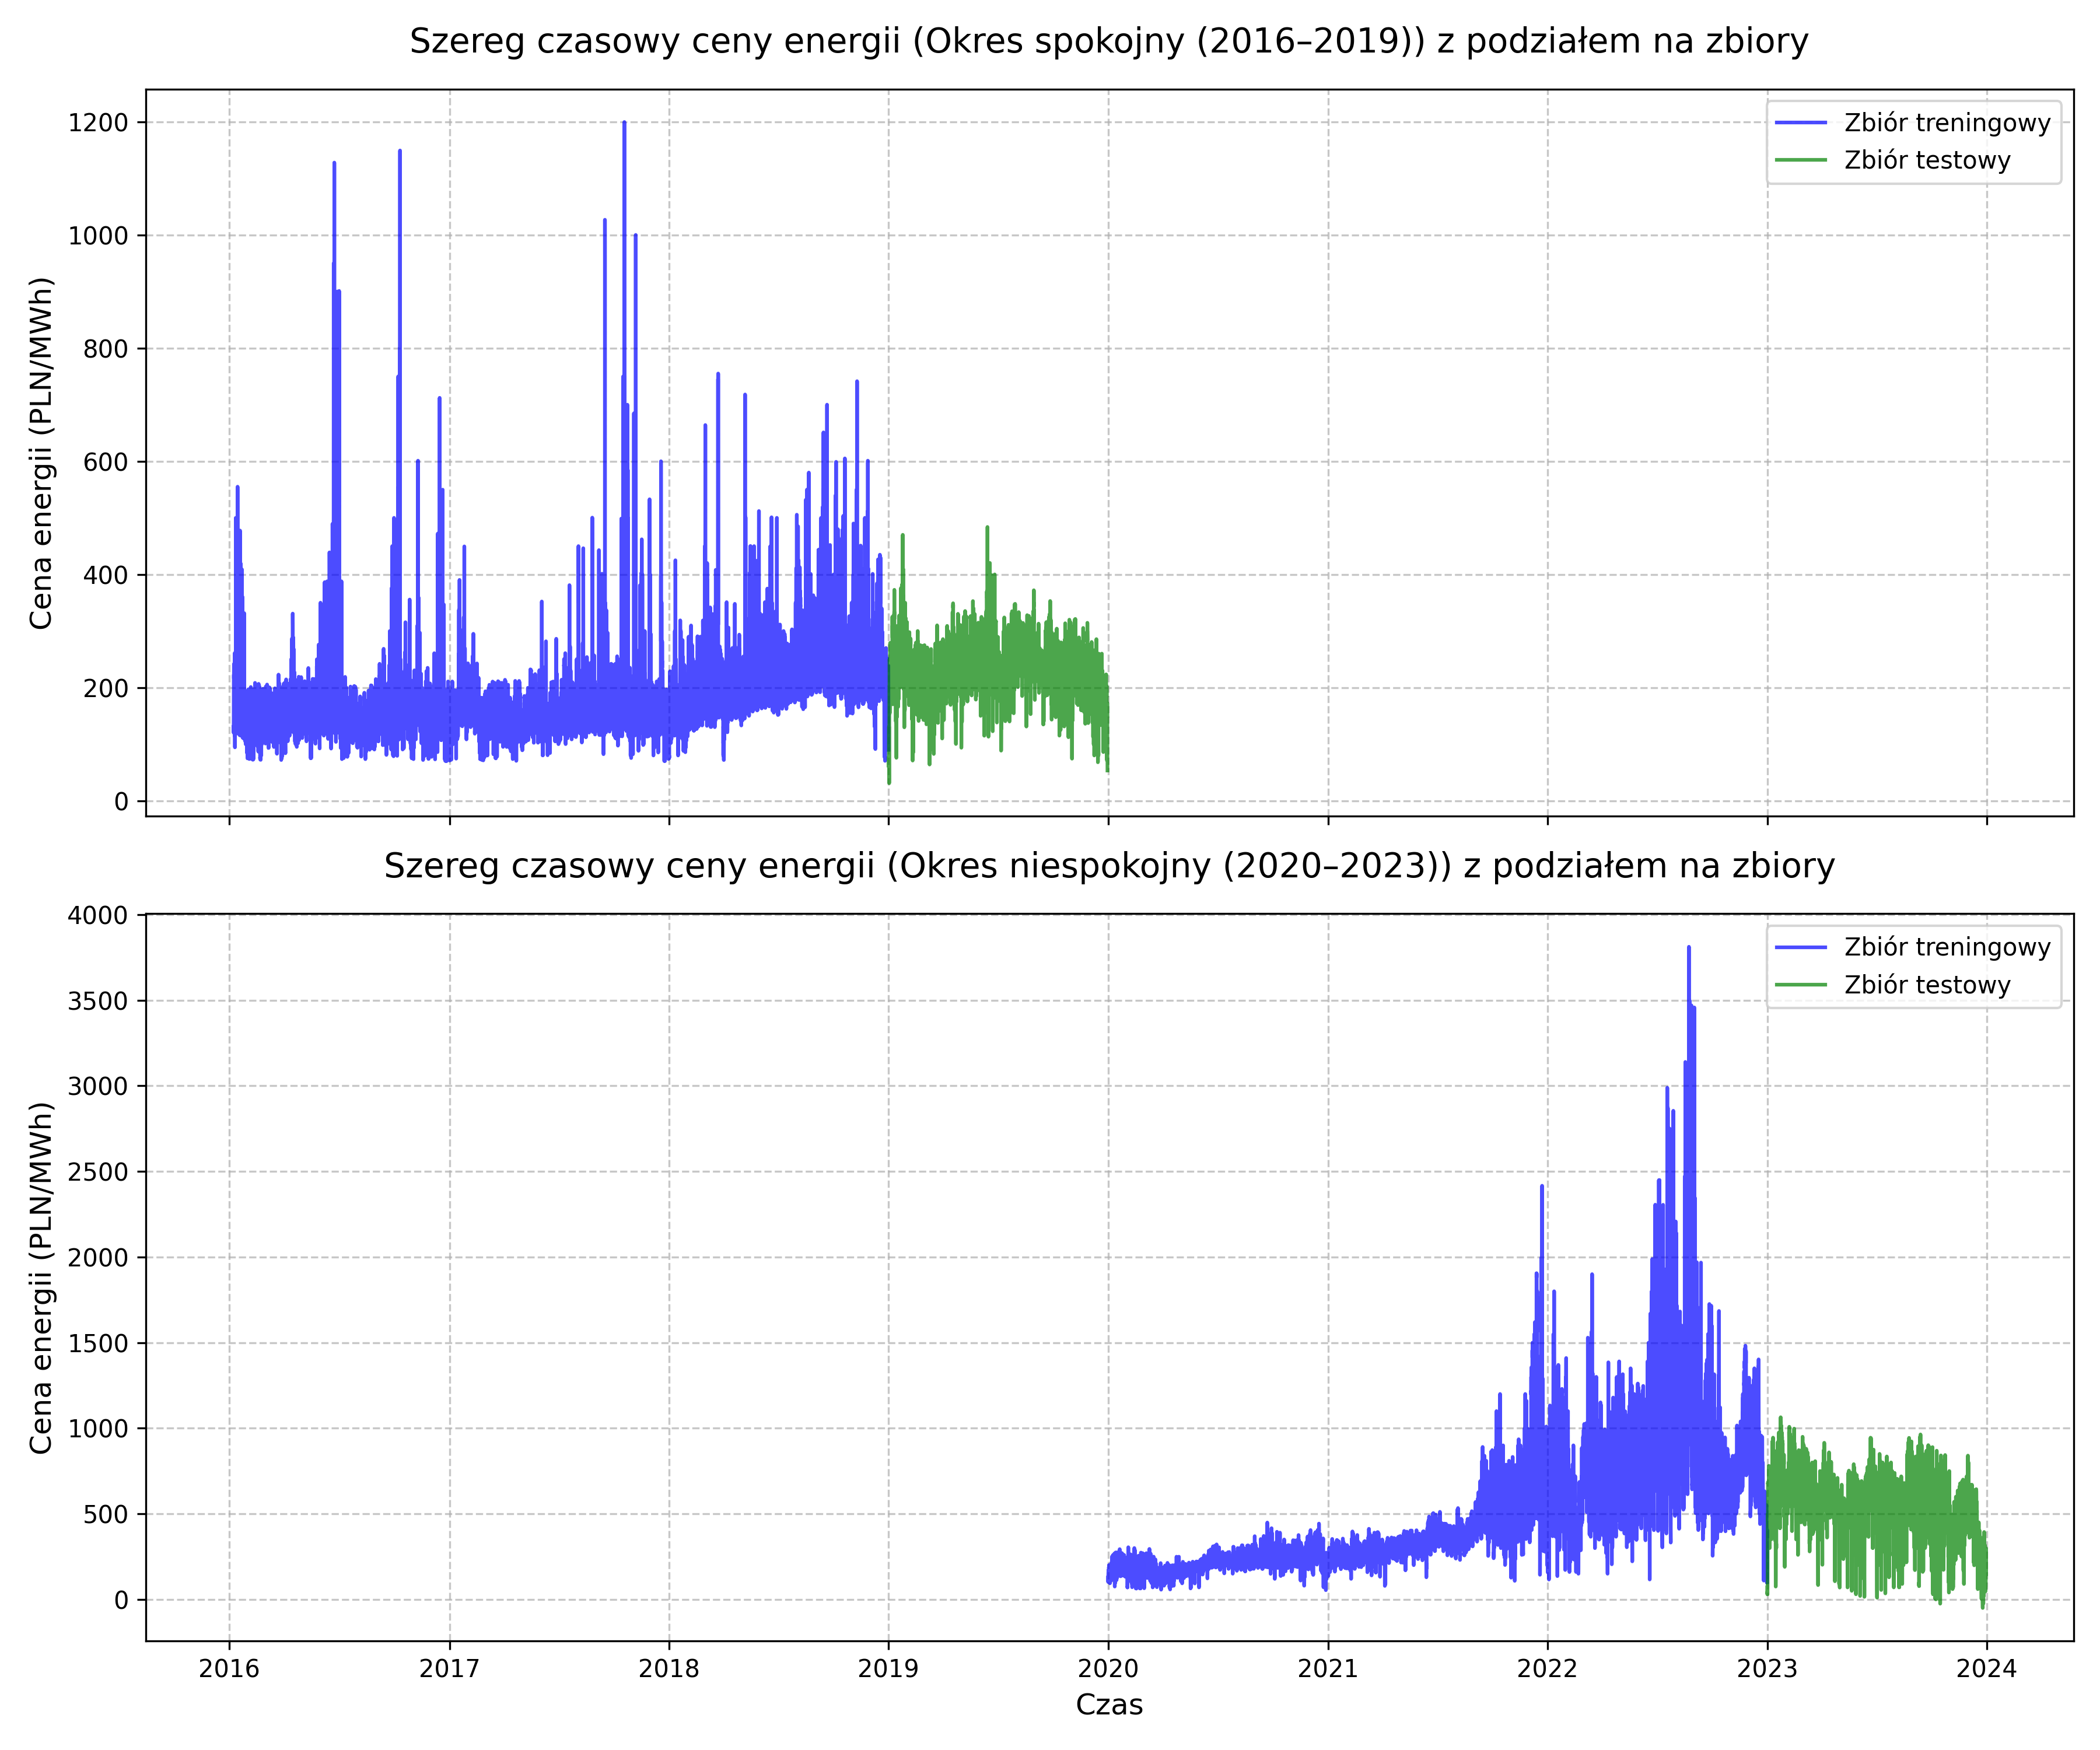
\includegraphics[width=0.9\textwidth]{../../plots/periods_split_combined.png}
    \caption{Podział szeregów czasowych cen energii na zbiory treningowe i testowe. Opracowanie własne.}
    \label{fig:periods_split_combined}
\end{figure}

\section{Przygotowanie danych}

Przed przystąpieniem do modelowania dane zostały poddane szeregu kroków preprocessingu, aby zapewnić ich odpowiednią jakość i format dla wybranych modeli.

Pierwszym krokiem jest kodowanie zmiennych cyklicznych. Zmienne sezonowe mają charakter cykliczny (np. po godzinie 23 następuje 0, po grudniu następuje styczeń). Aby uwzględnić tę cykliczność, zastosowano kodowanie za pomocą funkcji sinusoidalnych:

\begin{itemize}
    \item Dla \texttt{day\_of\_week}: \(\sin\left(\frac{2\pi \cdot \text{day\_of\_week}}{7}\right)\),
    \item Dla \texttt{month}: \(\sin\left(\frac{2\pi \cdot \text{month}}{12}\right)\),
    \item Dla \texttt{hour}: \(\sin\left(\frac{2\pi \cdot \text{hour}}{24}\right)\).
\end{itemize}

Oryginalne zmienne zostały usunięte, a ich zakodowane wersje dodano do zbioru danych. Kodowanie sinusoidalne pozwala modelom lepiej uchwycić cykliczność danych, w przeciwieństwie do kodowania typu one-hot, które zwiększyłoby wymiarowość danych i nie uwzględniało cykliczności.

Następnie, wszystkie zmienne numeryczne niebinarne zostały poddane standaryzacji StandardScaler z biblioteki \texttt{sklearn}. Standaryzacja polega na przekształceniu zmiennych, aby miały średnią 0 i odchylenie standardowe 1. Wartości zmiennych zostały przekształcone według wzoru:
\[ z = \frac{x - \mu}{\sigma}, \]
gdzie \( z \) to wartość po standaryzacji, \( x \) to wartość przed standaryzacją, \( \mu \) to średnia zmiennej, a \( \sigma \) to odchylenie standardowe. 

Standaryzacja jest kluczowym krokiem w preprocessingu danych, ponieważ większość algorytmów uczenia maszynowego zakłada, że dane mają podobną skalę. W przeciwnym razie algorytmy mogą być wrażliwe na różnice w skali zmiennych, co prowadzi do nieoptymalnych wyników. Proces standaryzacji został przeprowadzony osobno dla każdego z okresów spokojnego i niespokojnego osobno, aby uwzględnić różnice w rozkładach danych między tymi okresami. W obrębie każdego okresu parametry standaryzacji (średnia i odchylenie standardowe) obliczono na zbiorze treningowym i zastosowano zarówno do danych treningowych, jak i testowych, aby uniknąć wycieku informacji.

Wartości odstające (np. ekstremalnie wysokie ceny w okresie niespokojnym, takie jak 3812,45 PLN/MWh) nie zostały zmodyfikowane, ponieważ odzwierciedlają rzeczywiste zjawiska rynkowe (np. kryzys energetyczny w 2022 roku). Ich wpływ na modele będzie monitorowany podczas analizy wyników.
